% !TEX program = pdflatex
\documentclass{beamer}
\usepackage{iftex}
% This talk MUST be compiled with pdflatex.  Under lualatex/xelatex the
% "literate" replacements below never fire, and listings additionally sorts the
% Unicode characters into a different output buffer than the ASCII punctuation,
% which silently REORDERS the Lean code (e.g. "(⟨(‖p‖⁻¹" came out as "⟨‖((‖⁻p¹").
\ifpdftex
  \usepackage[T1]{fontenc}
  \usepackage[utf8]{inputenc}
\else
  \GenericError{}{Compile this file with pdflatex: listings garbles the Lean
    Unicode symbols under lualatex/xelatex.}{}{}
\fi
\usepackage{listings}
\usepackage{textcomp}
\usepackage{upquote} % Lean's ' (HEP', '') must print straight, not as a curly ’
\usepackage{amssymb}
\usepackage{xcolor}
\usepackage{upgreek}
\usepackage{mathtools}
\usepackage{graphicx}
\graphicspath{ {./images/} }

\usepackage[style=alphabetic,backend=biber]{biblatex}
\addbibresource{../thesis/Literatur.bib}
% Literaturangaben in Beamer nicht schrumpfen lassen
\setbeamerfont{bibliography item}{size=\footnotesize}
\setbeamerfont{bibliography entry author}{size=\footnotesize}
\setbeamerfont{bibliography entry title}{size=\footnotesize}
\setbeamerfont{bibliography entry location}{size=\footnotesize}
\setbeamerfont{bibliography entry note}{size=\footnotesize}
\setbeamertemplate{bibliography item}[text]

\usetheme{Berlin}
\usecolortheme{seahorse}

% Lean-Syntaxdefinition fuer listings
\lstdefinelanguage{Lean}{
  morekeywords={def,theorem,lemma,Prop,Set,Type,fun,let,in,if,then,else,
    match,with,structure,instance,class,where,by,do,Continuous,ContinuousOn,
    MapsTo,True,False,forall,exists},
  sensitive=true,
  morecomment=[l]{--},
  morecomment=[s]{/-}{-/},
  morestring=[b]",
}

\lstset{
  language=Lean,
  basicstyle=\ttfamily\scriptsize,
  keywordstyle=\color{blue!70!black}\bfseries,
  commentstyle=\color{gray}\itshape,
  stringstyle=\color{green!50!black},
  breaklines=true,
  showstringspaces=false,
  extendedchars=true,
  columns=fullflexible,
  keepspaces=true,
}

% Every Lean glyph used in the listings gets a math replacement.  Each entry MUST
% cover exactly ONE source character: a literate key that chains two non-ASCII
% characters (e.g. {⁻¹} or {↓∩}) makes inputenc abort with
% "Invalid UTF-8 byte sequence".  Multi-character symbols are therefore built up
% from their parts (⁻ then ¹ gives ⁻¹, ↓ then ∩ gives ↓∩, ≃ then ₜ gives ≃ₜ).
\lstset{literate=
  {·}{{$\cdot$}}1          % U+00B7  focus dot in tactic proofs
  {¹}{{$^{1}$}}1           % U+00B9
  {×}{{$\times$}}1         % U+00D7
  {‖}{{$\Vert$}}1          % U+2016  norm
  {•}{{$\bullet$}}1        % U+2022  scalar multiplication
  {⁻}{{$^{-}$}}1           % U+207B
  {ₜ}{{$_{\mathrm{t}}$}}1  % U+209C
  {ℕ}{{$\mathbb{N}$}}1     % U+2115
  {ℝ}{{$\mathbb{R}$}}1     % U+211D
  {→}{{$\rightarrow$}}1    % U+2192
  {↓}{{$\downarrow$}}1     % U+2193
  {↔}{{$\leftrightarrow$}}1% U+2194
  {↦}{{$\mapsto$}}1        % U+21A6
  {∀}{{$\forall$}}1        % U+2200
  {∃}{{$\exists$}}1        % U+2203
  {∈}{{$\in$}}1            % U+2208
  {∧}{{$\wedge$}}1         % U+2227
  {∨}{{$\vee$}}1           % U+2228
  {∩}{{$\cap$}}1           % U+2229
  {≃}{{$\simeq$}}1         % U+2243
  {≤}{{$\leq$}}1           % U+2264
  {⊆}{{$\subseteq$}}1      % U+2286
  {⟨}{{$\langle$}}1        % U+27E8
  {⟩}{{$\rangle$}}1        % U+27E9
  % not currently used, kept for future slides
  {¬}{{$\neg$}}1
  {∪}{{$\cup$}}1
  {∅}{{$\emptyset$}}1
  {∂}{{$\partial$}}1
  {⊤}{{$\top$}}1
  {↑}{{$\uparrow$}}1
  {⟶}{{$\longrightarrow$}}1
  {≥}{{$\geq$}}1
  {≠}{{$\neq$}}1
}

\usepackage{tikz}
\usetikzlibrary{shapes.geometric, arrows.meta, positioning}

% Definition der Kasten-Stile
\tikzstyle{box} = [
    rectangle,
    draw=black,
    thick,
    fill=blue!20,
    text width=2.5cm,
    text centered,
    rounded corners,
    minimum height=1.5cm
]
% iff pfeile
\tikzstyle{iffarrow} = [thick, {Stealth[scale=1.5]}-{Stealth[scale=1.5]}]

\title{Formalizing the Homotopy Extension Property}
\author{Mara Silge}
\date{16th July 2026}

% Zwischenfolie zu Beginn jeder Section: aktuelles Kapitel hervorgehoben,
% die uebrigen ausgegraut
\AtBeginSection[]{
\begin{frame}
\frametitle{Table of Contents}
\tableofcontents[currentsection]
\end{frame}
}

\begin{document}

%Titelseite
\begin{frame}
\titlepage
\end{frame}

% Inhaltsverzeichniss
\begin{frame}
\frametitle{Table of Contents}
\tableofcontents
\end{frame}


\section{Motivation}
\begin{frame}
\frametitle{Goals of the thesis}
\begin{itemize}
\item defining the homotopy extension property in Lean
\item tools to prove the homotopy extension property
\begin{itemize}
\item retraction criterion
\item homeomorphic space pairs inherit the homotopy extension property from one another
\end{itemize}
\item proving the homotopy extension property for relative CW-complexes
\end{itemize}
\end{frame}

\begin{frame}
\frametitle{Motivation}
\begin{theorem}[Cellular Approximation Theorem, {\cite[Theorem 4.8]{HAT01}}] 
    Every map $f \colon X \to Y $ of CW complexes is homotopic to a cellular map. If $f$ is already cellular on a subcomplex $A \subset X$, the homotopy may be taken to be stationary on A.
\end{theorem}
\begin{theorem}[Whitehead's Theorem, {\cite[Theorem 4.5]{HAT01}}] 
    If a map $f \colon X \to Y$ between connected CW complexes induces isomorphisms $f_* \colon \pi_n (X) \to  \pi _n (Y) $ for all $n$, then $f$ is a homotopy equivalence. 
\end{theorem}
\end{frame}


\section{Mathematics of the Homotopy Extension Property}

\begin{frame}[shrink=5]
\frametitle{The Homotopy Extension Property}
Remark: All maps of topological spaces are assumed to be continuous.
\begin{definition}[Homotopy Extension Property (HEP) \cite{JHU}]\label{HEP}
A pair of topological spaces $(X,A)$ with $A \subseteq X$ has the
\emph{homotopy extension property (HEP)} if for every topological space $Y$, every
map $f \colon X \to Y$, and every homotopy $H \colon A \times [0,1] \to Y$ satisfying
$H(a,0) = f(a)$ for all $a \in A$, there exists a homotopy
$H' \colon X \times [0,1] \to Y$ such that
\begin{align*}
    H'(x,0) &= f(x)    && \text{for all } x \in X, \\
    H'(a,t) &= H(a,t)  && \text{for all } (a,t) \in A \times [0,1].
\end{align*}
\end{definition}
\begin{itemize}
\item $(X,X)$ has the HEP
\item $(X, \emptyset )$ has the HEP
\end{itemize}
\end{frame}

\begin{frame}
\frametitle{Retraction}
Let $(X,A)$ be a pair of topological spaces with $A \subseteq X$.
\begin{definition}[Retraction]
A map $r \colon X \to A$ is a \emph{retraction} if $r \circ \mathrm{incl}_A = \mathrm{id}_A$.
\end{definition}
Equivalently, the function $r \colon X \to A$
\begin{itemize}
\item is continuous,
\item is fixed on $A$, i.e.\ $r(a) = a$ for all $a \in A$.
\end{itemize}
\end{frame}

\begin{frame}
\frametitle{Retraction Criterion}
\begin{lemma}[Retraction Criterion]
Let $X$ be a topological space, $A \subseteq X$ a subspace.
Consider the following two statements:
\begin{enumerate}
    \item The pair $(X,A)$ has the \emph{HEP}.
    \item The subspace $(X \times \{0\}) \cup (A \times [0,1])$ is a retract of $X \times [0,1]$.
\end{enumerate}
Then $(1) \implies (2)$. If, in addition, $A$ is closed in $X$, the converse
$(2) \implies (1)$ holds as well.
\end{lemma}
\end{frame}


\begin{frame}
\frametitle{Retraction Criterion}
Let $X$ be a topological space and $A \subseteq X$ a closed subspace.
\begin{center}
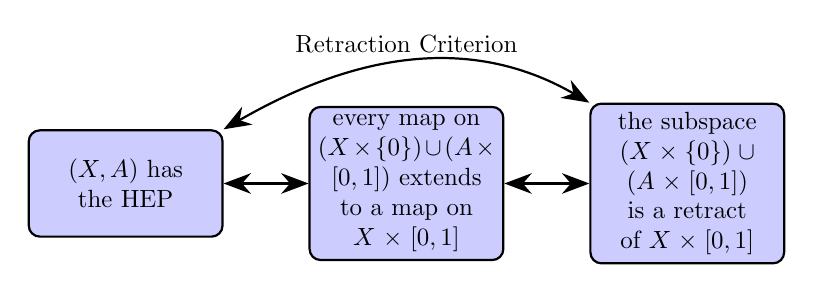
\begin{tikzpicture}[node distance=1.2cm, auto, scale=0.9, transform shape]
    % Kästen definieren
    \node (box1) [box] {$(X,A)$ has the HEP};
    \node (box2) [box, right=of box1] {every map on $(X \times \{0\}) \cup (A \times [0,1])$ extends to a map on $X \times [0,1]$};
    \node (box3) [box, right=of box2] {the subspace $(X \times \{0\}) \cup (A \times [0,1])$ is a retract of $X \times [0,1]$};
    % Pfeile
    \draw [iffarrow] (box1) -- (box2);
    \draw [iffarrow] (box2) -- (box3);
    \draw [iffarrow] (box1.north east) to [out=30, in=150] node[above] {Retraction Criterion} (box3.north west);
\end{tikzpicture}
\end{center}
\end{frame}

\begin{frame}
\frametitle{HEP for relative CW-complexes}
Let $X$ be a CW-complex with skeleta $(X_n)_{n \in \mathbb{N}}$. \\
Strategy:
\begin{enumerate}
    \item Any disc relative to its boundary has the \emph{HEP}.
    \item The pair of two consecutive skeleta has the \emph{HEP}, i.e.\ $(X_{n+1},X_n)$ has the \emph{HEP} for all $n$.
    \item Any relative CW-complex has the \emph{HEP}.
\end{enumerate}
\end{frame}

\begin{frame}
\frametitle{HEP for discs/cubes relative boundary}
\begin{theorem} [\cite{JHU}]
The pair $(D^m, S^{m-1})$ has the \emph{HEP} for all $m \in \mathbb{N}$.
\end{theorem} \pause
\begin{theorem}
    The \emph{HEP} is preserved under homeomorphisms: let $(X,A)$ and $(Y,B)$ be space pairs. If there exists a homeomorphism from $X$ to $Y$ that maps $A$ to $B$, and $(X,A)$ has the \emph{HEP}, then so does $(Y,B)$.
\end{theorem} \pause
\begin{theorem}
The pair $([0,1]^m, \partial ([0,1]^m))$ has the \emph{HEP} for all $m \in \mathbb{N}$.
\end{theorem} 
\end{frame}


\section{Formalization in Lean}

\begin{frame}[fragile]
\frametitle{Definition of the HEP (1/2)}
\begin{itemize}\footnotesize
\item \texttt{agreeOn} isolates the compatibility condition $H(a,0) = f(a)$
\item homotopies have type $X \times \mathbb{R} \to Y$, not $A \times [0,1] \to Y$
\item \texttt{HomotopyExtension} $\colon$ exactly the three conditions of the desired homotopy
\end{itemize}
\begin{lstlisting}
universe u
variable {X Y : Type u} [TopologicalSpace X] [TopologicalSpace Y] {A : Set X}

def agreeOn (f : X → Y) (H : X × ℝ → Y) (A : Set X) : Prop := ∀ (a : A), f a = H (a,0)

def HomotopyExtension (H' : X × ℝ → Y) (f : X → Y) (H : X × ℝ → Y) (A : Set X) :
    Prop :=
  ContinuousOn H' { p : X × ℝ | p.2 ∈ unitInterval} ∧
  (∀ (x : X), f x = H' (x, 0)) ∧ (∀ (a : A) (t : unitInterval), H (a,t) = H' (a, t))
\end{lstlisting}
\end{frame}

\begin{frame}[fragile]
\frametitle{Definition of the HEP (2/2)}
\begin{lstlisting}
def HEP (X : Type u) [TopologicalSpace X] (A : Set X) : Prop :=
  ∀ (Y : Type u) [TopologicalSpace Y], ∀ (f : X → Y), 
  ∀ (H : X × ℝ → Y), Continuous f → 
  ContinuousOn H {p : X × ℝ | (p.1 ∈ A) ∧ (p.2 ∈ (unitInterval))} → 
  agreeOn f H A → ∃ (H' : X × ℝ → Y), HomotopyExtension H' f H A
\end{lstlisting}
\end{frame}

\begin{frame}[fragile]
\frametitle{HEP for a subset instead of a subtype}
\begin{itemize}
\item motivation: in a CW-complex all skeleta $X_n$ are \emph{subsets} of one ambient space
\item \texttt{HEP\_HEP'}: the two formulations really are equivalent, so nothing is lost
\end{itemize}
\begin{lstlisting}
open Set.Notation

def HEP' {Y : Type*} [TopologicalSpace Y] (X A : Set Y) : Prop := 
  HEP X (X ↓∩ A)

lemma HEP_HEP' {Y : Type*} [TopologicalSpace Y] (X : Set Y) 
    (A : Set (Set.Elem X)) : 
    HEP (X.Elem) A ↔ HEP' X (Subtype.val '' A) := by
  unfold HEP'
  rw [Set.preimage_val_image_val_eq_self]
\end{lstlisting}
\end{frame}

\begin{frame}[fragile]
\frametitle{Retraction Criterion in Lean}
\begin{lstlisting}
structure RetractionOn {X : Type*} [TopologicalSpace X] 
    (r : X → X) (B A : Set X) : Prop where
  subset : A ⊆ B
  continuousOn : ContinuousOn r B
  mapsTo : B.MapsTo r A
  fixesOn : ∀ a ∈ A, r a = a

lemma retraction_criterion_closed (hA1 : IsClosed A) :
    HEP X A ↔ ∃ r : X × ℝ → X × ℝ, 
    RetractionOn r {p : X × ℝ | p.2 ∈ unitInterval}
    {p : X × ℝ | p.2 = 0 ∨ (p.1 ∈ A) ∧ p.2 ∈ unitInterval}

lemma retraction_criterion_closed' {Y : Type u} [TopologicalSpace Y] (A X : Set Y) (hAX : A ⊆ X)
    (hA1 : IsClosed A) : HEP' X A ↔ ∃ r : Y × ℝ → Y × ℝ, RetractionOn r
    {p : Y × ℝ | p.1 ∈ X ∧ p.2 ∈ unitInterval}
    {p : Y × ℝ | p.1 ∈ X ∧ p.2 = 0 ∨ (p.1 ∈ A) ∧ p.2 ∈ unitInterval}
\end{lstlisting}
\end{frame}

\begin{frame}[fragile]
\frametitle{Transport along a partial homeomorphism}
\begin{itemize}
\item global homeomorphism $X \simeq Y$ would be stronger
\item HEP' is more usfull for partial homeomorphism
\item subspaces have to be closed to apply the retraction criterion
\end{itemize}
\begin{lstlisting}
lemma PartialHomeomorph_HEP' {X Y : Type*} [TopologicalSpace X] 
  [TopologicalSpace Y] {X1 X2 : Set X} (hX : X2 ⊆ X1) {Y1 Y2 : Set Y} 
  (hY : Y2 ⊆ Y1) (hHEP : HEP' X1 X2) (f : PartialHomeomorph X Y) 
  (hf_source : f.source = X1) (hf_target : f.target = Y1)
  (h2 : f '' X2 = Y2) (hX2closed : IsClosed (X2 : Set X)) 
  (hY2closed : IsClosed (Y2 : Set Y)) : HEP' Y1 Y2
\end{lstlisting}
\end{frame}

\begin{frame}[fragile]
\frametitle{HEP for the disc relative to its boundary}
\begin{itemize}
\item \texttt{use H'}: explicitly constructed earlier
\item the primed version follows by \texttt{exact}: both statements are definitionally equal
\end{itemize}
\begin{lstlisting}
lemma HEP_disc_boundary : ∀ (m : ℕ),
    HEP (Metric.closedBall (0 : EuclideanSpace ℝ (Fin m)) 1) (Metric.sphere ⟨0, by simp⟩ 1):= by
  intro m Y hY f H hf_cont hH_cont hAgree
  use H' f H
  refine ⟨?_ , ?_ , ?_ ⟩
  · exact H'_ContinuousOn f H hf_cont hH_cont hAgree
  · intro x
    simp [H', aux_fun, mem_closedBall_zero_iff.mp x.prop]
  · exact H'_agreeH f H hAgree

lemma HEP_disc_boundary' : ∀ (m : ℕ),
    HEP' (Metric.closedBall (0 : EuclideanSpace ℝ (Fin m)) 1) (Metric.sphere 0 1):= by
  exact HEP_disc_boundary
\end{lstlisting}
\end{frame}


\begin{frame}[fragile, shrink = 5]
\frametitle{From the disc to the cube}
\begin{center}
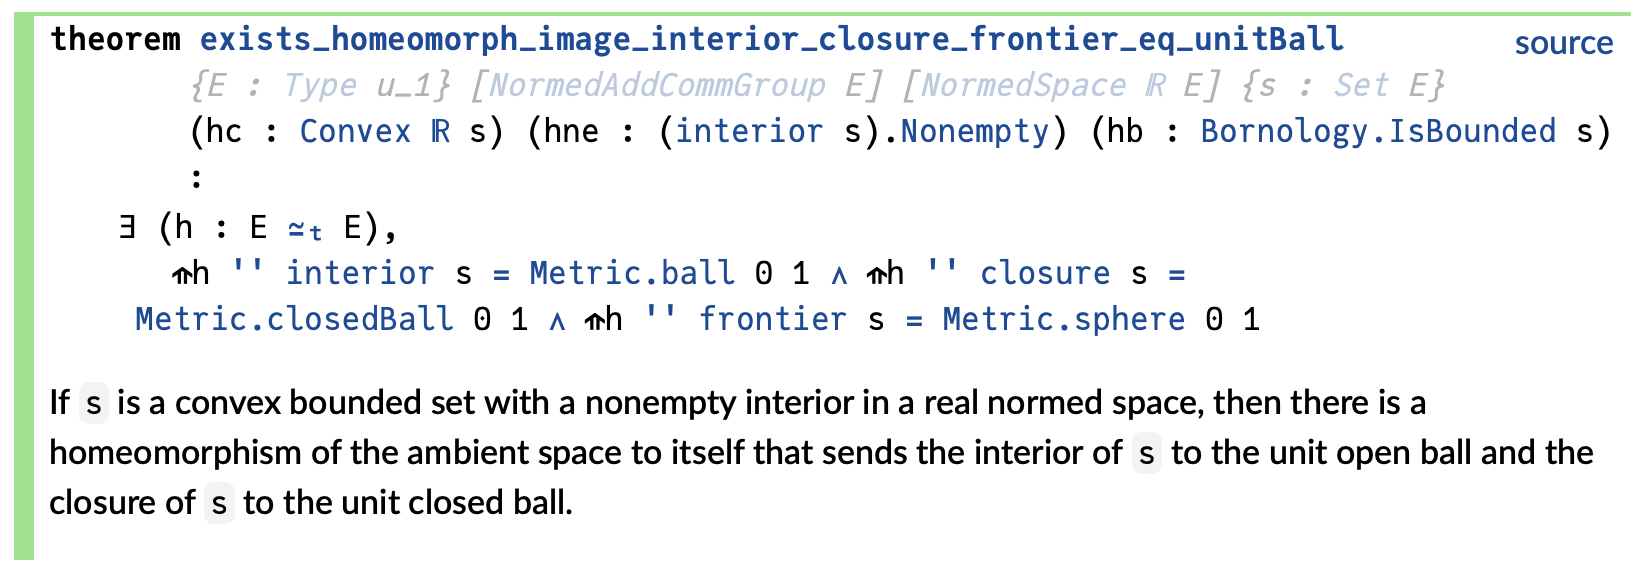
\includegraphics[width=\textwidth]{image_homeo.png}
\end{center}
\begin{itemize}\footnotesize
\item \texttt{EuclideanSpace} carries the $\ell^2$-norm, the type $\mathrm{Fin}\ m \to \mathbb{R}$ the $\ell^\infty$-norm
\item the above lemma matches closure with closure and frontier with frontier
\end{itemize}
\begin{lstlisting}
def fun_euclid_max : EuclideanSpace ℝ (Fin m) → (Fin m → ℝ) := fun p ↦ p

def G : (Fin m → ℝ) ≃ₜ (Fin m → ℝ):= (exists_homeomorph_image_interior_closure_frontier_eq_unitBall
  convex_euclid_to_max_ball
  nonempty_euclid_to_max_ball bounded_euclid_to_max_ball).choose
\end{lstlisting}
\end{frame}



\appendix
\begin{frame}[allowframebreaks]
\frametitle{References}
\printbibliography[heading=none]

\vfill
\footnotesize
Formalisation and slides:
\url{https://github.com/marasilge/Bachelorarbeit}
\end{frame}


\end{document}